\chapter{Przedmiot pracy: projekt i implementacja systemu transkrypcji gitarowej}
\label{chap:przedmiot_pracy}

Przyjęta w~ramach tej pracy strategia, polegająca na bezpośredniej predykcji progów gitarowych, jest wynikiem analizy i~badań eksploracyjnych nad alternatywnymi podejściami. Wstępna faza projektu obejmowała próby adaptacji istniejących, zaawansowanych modeli transkrypcji polifonicznej, w~szczególności modelu Basic Pitch (w literaturze określanego jako NMP~– Notes and Multipitch)~\autocite{Bittner2022BasicPitch} oraz koncepcji ,,Onsets and Frames''~\autocite{Hawthorne2018Onsets}. Celem tych eksperymentów było zbadanie, czy modele zoptymalizowane do ogólnej transkrypcji (predykcji nut i~onsetów) można z~powodzeniem wyspecjalizować do zadania generowania tabulatur (GTT) wyłącznie na zbiorze danych GuitarSet.

Doświadczenia te, choć nie przyniosły zadowalających rezultatów w~postaci gotowego rozwiązania, dostarczyły kluczowych wniosków. Stwierdzono, że skuteczność referencyjnych architektur jest silnie uzależniona od treningu na bardzo dużych i~zróżnicowanych zbiorach danych (takich jak MAESTRO czy Slakh), a~ich ograniczenie wyłącznie do specyfiki GuitarSet okazało się niewystarczające. Analiza wykazała, że zarówno modele agnostyczne instrumentalnie, jak i~podejścia dwuetapowe (predykcja nut, a~następnie inferencja tabulatury) mają trudności z~uchwyceniem subtelnych zależności niezbędnych do poprawnego mapowania dźwięków na konkretne struny i~progi. Wnioski te jednoznacznie wskazały na konieczność opracowania dedykowanego modelu, uczącego się bezpośredniej predykcji tabulatury, co stało się fundamentem rozwiązania przedstawionego w~dalszej części niniejszego rozdziału.

Niniejszy rozdział stanowi szczegółowe omówienie projektu i~implementacji autorskiego systemu do GTT. Celem prac było stworzenie oraz ewaluacja systemu zdolnego do przekształcania sygnału audio gitary w~symboliczną reprezentację tabulaturową, z~wykorzystaniem technik DL. Kluczowym aspektem projektu jest możliwość eksperymentalnego porównania dwóch odmiennych metod reprezentacji sygnału wejściowego: tradycyjnych mel-spektrogramów oraz transformaty CQT, celem zbadania ich efektywności w~zadaniu GTT. Opierając się na fundamentach teoretycznych i~przeglądzie stanu wiedzy przedstawionym w~poprzednich rozdziałach, w~tej części pracy opisana zostanie architektura i~logika działania opracowanego rozwiązania. Prezentacja ta ma na celu nie tylko techniczny opis zrealizowanych prac, ale również analityczne osadzenie podjętych decyzji projektowych w~kontekście literatury naukowej.

\section{Analiza teoretyczna rozwiązania}
\label{sec:analiza_teoretyczna_rozwiazania_fakt}

W tej sekcji dokonano analizy teoretycznej zaimplementowanego systemu, odnosząc poszczególne komponenty do ugruntowanych koncepcji teoretycznych i~literatury naukowej, co stanowi uzasadnienie dla podjętych decyzji projektowych.

\subsection{Wykorzystany zbiór danych: GuitarSet}
\label{ssec:analiza_guitarset}

Prezentowane badania oparto na publicznie dostępnym zbiorze danych GuitarSet~\autocite{Xi2018}. Jego wybór był podyktowany unikalnymi cechami technicznymi, które czynią go kluczowym i~wszechstronnym zasobem w~badaniach nad automatyczną transkrypcją gitarową (GTT), a~w~szczególności nad problemem niejednoznaczności opalcowania. Od momentu publikacji, GuitarSet stał się de facto standardem i~podstawowym zbiorem benchmarkowym, służącym do ewaluacji i~porównywania nowych modeli w~dziedzinie analizy muzyki gitarowej.

GuitarSet składa się z~360 trzydziestosekundowych fragmentów audio, nagranych przez sześciu różnych gitarzystów na gitarze akustyczno-elektrycznej. Zbiór charakteryzuje się starannie zaplanowaną strukturą, zapewniającą dużą różnorodność muzyczną. Każdy muzyk nagrał ten sam zestaw 30 partii, obejmujących dwa style wykonania (akompaniament oraz solo), pięć gatunków muzycznych (rock, jazz, funk, bossa nova, styl piosenki autorskiej) oraz trzy progresje akordów (dwunastotaktowy blues, ,,Autumn Leaves'' i~Kanon Pachelbela), wykonane w~dwóch różnych tempach. Taka konstrukcja zapewnia szerokie spektrum kontekstów muzycznych i~technik gry.

Kluczowym elementem, który wyróżnia GuitarSet, jest metoda rejestracji sygnału. Każda z~sześciu strun gitary została wyposażona w~osobny przetwornik heksafoniczny, co pozwoliło na nagranie sygnału z~każdej struny niezależnie. Równocześnie z~nagraniem heksafonicznym, dźwięk rejestrowano za pomocą wysokiej jakości mikrofonu pojemnościowego. W~rezultacie zbiór udostępnia dane audio w~czterech wariantach:
\begin{itemize}
    \item \texttt{audio\_hex-pickup\_original}: surowe, 6-kanałowe nagrania z~przetwornika heksafonicznego, zawierające naturalne przesłuchy międzykanałowe.
    \item \texttt{audio\_hex-pickup\_debleeded}: wersja powyższych nagrań poddana cyfrowej obróbce w~celu usunięcia przesłuchów, co skutkuje niemal idealną separacją sygnału dla każdej struny.
    \item \texttt{audio\_mono-pickup\_mix}: monofoniczny miks sygnałów z~przetwornika heksafonicznego, symulujący standardowe wyjście liniowe gitary.
    \item \texttt{audio\_mono-mic}: monofoniczne nagranie z~mikrofonu, reprezentujące najbardziej realistyczny, a~zarazem najtrudniejszy scenariusz dla algorytmów GTT.
\end{itemize}

Wykorzystanie nagrań heksafonicznych drastycznie uprościło proces adnotacji, który w~dużej mierze mógł zostać zautomatyzowany, a~następnie poddany jedynie ręcznej weryfikacji i~korekcie. Pozwoliło to na osiągnięcie niespotykanej dotąd precyzji na dużą skalę. Adnotacje, dostępne w~formacie JAMS (JSON Annotated Music Specification), są wyjątkowo bogate. Dla każdej nuty zawierają one nie tylko jej wysokość, czas rozpoczęcia i~czas trwania, ale również~– co jest unikalne na tle innych zbiorów~– dokładną informację o~strunie i~progu, na których została zagrana~\autocite{Wiggins2019TabCNN, Xi2018}. Ponadto zbiór zawiera kontury wysokości dźwięku dla każdej struny, pozycje uderzeń rytmicznych (beat) oraz dwa rodzaje adnotacji harmonicznych: akordy, które muzyk miał zagrać (z nut), oraz te, które faktycznie zagrał (wywnioskowane na podstawie analizy wykonania).

Ta szczegółowa struktura danych jest niezbędna do trenowania i~wiarygodnej ewaluacji modeli GTT, które mają za zadanie nauczyć się nie tylko ,,co'' zostało zagrane, ale również ,,jak'' i~,,gdzie'' na gryfie gitary. Wszechstronność zbioru sprawia, że jest on wykorzystywany również w~innych zadaniach badawczych, takich jak analiza stylu gry, rozpoznawanie zaawansowanych technik artykulacyjnych czy klasyfikacja gatunków muzycznych. Mimo relatywnie niewielkiego rozmiaru w~porównaniu do zbiorów danych dla innych instrumentów (np. MAESTRO dla fortepianu), GuitarSet pozostaje fundamentalnym zasobem w~swojej dziedzinie. Należy jednak zaznaczyć, że w~ramach przygotowania danych do treningu, zgodnie z~doniesieniami społeczności, ze zbioru wyłączono dwa pliki: \texttt{04\_BN3-154-E\_comp} oraz \texttt{04\_Jazz1-200-B\_comp}, ze względu na minimalne błędy w~synchronizacji czasowej adnotacji~\autocite{Riley2023GuitarSetIssue}.

\subsection{Wybór architektury CRNN w kontekście GTT}
\label{ssec:analiza_crnn_teoretyczna_fakt}

Zastosowanie architektury CRNN jest dobrze uzasadnione specyfiką zadania GTT. Połączenie CNN jako ekstraktora cech z~wejściowych reprezentacji czasowo-częstotliwościowych oraz RNN do modelowania sekwencji czasowych tych cech jest sprawdzonym podejściem w~dziedzinie transkrypcji muzycznej~\autocite{Hawthorne2018Onsets, Wiggins2019TabCNN}.
\begin{itemize}
    \item \textbf{Warstwy konwolucyjne (CNN)} efektywnie uczą się hierarchicznych, lokalnych cech z~dwuwymiarowych spektrogramów (Mel lub CQT). Są zdolne do identyfikacji wzorców istotnych dla rozpoznawania dźwięków gitarowych, takich jak struktury harmoniczne czy transjenty~\autocite{Wiggins2019TabCNN, Benetos2019AutomaticMusicTranscription}.
    \item \textbf{Warstwy rekurencyjne (RNN)}, w~tym przypadku dwukierunkowe, są wyspecjalizowane w~modelowaniu zależności czasowych w~sekwencjach cech dostarczonych przez CNN~\autocite{Benetos2019AutomaticMusicTranscription}. Dwukierunkowość pozwala na analizę każdej ramki w~kontekście zarówno przeszłych, jak i~przyszłych zdarzeń, co jest korzystne dla precyzji transkrypcji~\autocite{Hawthorne2018Onsets}. W~pracy testowano zarówno jednostki LSTM, jak i~GRU, które dzięki prostszej budowie mogą być bardziej efektywne obliczeniowo~\autocite{Chung2014GRU}.
\end{itemize}
Podejście wielozadaniowe, polegające na jednoczesnej predykcji onsetów i~progów przez oddzielne głowice wyjściowe, inspirowane pracą~\autocite{Hawthorne2018Onsets}, pozwala modelowi uczyć się bardziej kompletnych reprezentacji.

\subsection{Reprezentacja sygnału wejściowego}
\label{ssec:analiza_reprezentacji_teoretyczna_fakt}

System umożliwia eksperymentalne porównanie dwóch typów reprezentacji czasowo-częstotliwościowych, co stanowi istotny element badawczy.
\begin{itemize}
    \item \textbf{Mel-spektrogramy} są standardowym wyborem w~wielu zadaniach MIR ze względu na ich psychoakustyczną motywację – skala Mel aproksymuje ludzką percepcję wysokości dźwięku~\autocite{Benetos2019AutomaticMusicTranscription, KlapuriDavy2006SignalProcessing}.
    \item \textbf{Spektrogramy CQT} oferują logarytmiczne skalowanie osi częstotliwości, co bezpośrednio odpowiada strukturze skal muzycznych. Taka reprezentacja, gdzie rozdzielczość częstotliwościowa jest proporcjonalna do częstotliwości (np. stała liczba prążków na oktawę), może być bardziej naturalna dla modeli CNN w~zadaniach muzycznych, potencjalnie ułatwiając naukę cech niezmienniczych względem wysokości dźwięku~\autocite{Wiggins2019TabCNN, Zang2023SynthTab, KlapuriDavy2006SignalProcessing}.
\end{itemize}
Możliwość generowania CQT w~locie dla zbioru treningowego, w~połączeniu z~augmentacją audio, pozwala na efektywne wykorzystanie tej reprezentacji bez konieczności wstępnego przetwarzania i~przechowywania dużych ilości danych.

\subsection{Funkcja straty i optymalizacja wielozadaniowa}
\label{ssec:analiza_loss_teoretyczna_fakt}

Zastosowanie złożonej funkcji straty, będącej ważoną sumą strat dla predykcji onsetów i~progów, jest przykładem uczenia wielozadaniowego (ang. \textit{multi-task learning}). Takie podejście często prowadzi do poprawy jakości predykcji, ponieważ model uczy się współdzielonych reprezentacji, które są korzystne dla obu powiązanych zadań~\autocite{Hawthorne2018Onsets}.
\begin{itemize}
    \item Użycie binarnej entropii krzyżowej dla predykcji onsetów jest standardem dla zadań klasyfikacji binarnej.
    \item Użycie entropii krzyżowej dla predykcji progów jest odpowiednie dla zadań klasyfikacji wieloklasowej.
\end{itemize}
Maskowanie strat w~celu ignorowania dopełnionych części sekwencji oraz możliwość ważenia poszczególnych komponentów straty są istotnymi elementami zapewniającymi stabilny i~efektywny trening.

\subsection{Techniki augmentacji danych}
\label{ssec:analiza_augmentacji_teoretyczna_fakt}

Zastosowane techniki augmentacji danych odgrywają kluczową rolę w~procesie treningu, szczególnie przy pracy ze zbiorami danych o~ograniczonej wielkości, takimi jak GuitarSet~\autocite{Wiggins2019TabCNN, Zang2023SynthTab}. Rozbudowany zestaw augmentacji został wprowadzony w~odpowiedzi na niezadowalającą skuteczność modelu na nagraniach domowych. Przyjęta filozofia zakłada celowe wprowadzanie zakłóceń do idealnych danych treningowych, aby nauczyć model generalizacji do niedoskonałych warunków rzeczywistych.
\begin{itemize}
    \item \textbf{Augmentacje audio}, takie jak rozciąganie w~czasie, dodawanie szumu czy losowe wzmocnienie, symulują naturalne wariacje w~grze~\autocite{Su2014SparseCepstral, KlapuriDavy2006SignalProcessing}. Zostały one uzupełnione o~techniki modelujące specyficzne problemy nagrań amatorskich: symulacja pogłosu, zniekształceń charakterystyki mikrofonu czy cyfrowego przesterowania.
    \item \textbf{Augmentacja spektrogramu} (SpecAugment), polegająca na maskowaniu fragmentów w~dziedzinie czasu i~częstotliwości, zmusza model do nauki bardziej odpornych i~rozproszonych cech~\autocite{Zang2023SynthTab, Park2019SpecAugment}.
\end{itemize}
Stosowanie tych technik wyłącznie na zbiorze treningowym i~w~locie jest efektywnym sposobem na zwiększenie efektywnego rozmiaru zbioru treningowego bez konieczności generowania i~przechowywania dodatkowych danych.

\section{Opis zaimplementowanego rozwiązania}
\label{sec:rozwiazanie_dyplomanta}

Po przedstawieniu teoretycznych podstaw i~uzasadnieniu podjętych decyzji projektowych, niniejsza sekcja koncentruje się na szczegółowym opisie implementacji poszczególnych komponentów systemu.


\subsection{Architektura ogólna systemu}
\label{ssec:architektura_ogolna}

Zaproponowany system GTT charakteryzuje się modułową architekturą potokową (ang. \textit{pipeline}), co umożliwia elastyczne zarządzanie poszczególnymi etapami przetwarzania oraz systematyczne prowadzenie eksperymentów. Rozwiązanie zostało zaprojektowane w~taki sposób, aby oddzielić od siebie logikę poszczególnych komponentów, takich jak moduł przetwarzania danych, definicja modelu sieci neuronowej, procedura treningu oraz skrypty do ewaluacji i~analizy wyników.

Centralnym punktem sterującym jest interaktywny notatnik, który orkiestruje cały proces badawczy, jednak jego rola sprowadza się do wywoływania odpowiednich, niezależnych modułów. Za spójność i~powtarzalność eksperymentów odpowiada centralny mechanizm konfiguracyjny, który agreguje wszystkie globalne stałe i~parametry. Obejmują one definicje ścieżek dostępu do danych, parametry przetwarzania sygnału audio (takie jak częstotliwość próbkowania czy długość kroku analizy), specyficzne ustawienia dla generowania reprezentacji czasowo-częstotliwościowych (np. rozmiar okna FFT, liczba pasm Mel, liczba prążków dla CQT), a~także hiperparametry modelu i~procesu treningu. Taka struktura ułatwia modyfikację i~zapewnia spójność w~całym systemie.

%%
\subsection{Przetwarzanie wstępne i przygotowanie danych}
\label{ssec:przetwarzanie_wstepne_dane}

Staranne przygotowanie danych jest fundamentalnym etapem w~procesie uczenia maszynowego. W~ramach systemu obejmuje ono podział zbioru danych, ekstrakcję cech akustycznych z~plików audio, przetwarzanie adnotacji oraz zapis przetworzonych danych w~formacie tensorów.

\subsubsection{Podział zbioru danych}
\label{sssec:podzial_zbioru}

Jak szczegółowo opisano w~sekcji~\ref{ssec:analiza_guitarset}, badania oparto na zbiorze danych GuitarSet. Po wykluczeniu dwóch problematycznych plików, pozostało 358 nagrań do dyspozycji. Zbiór ten został podzielony w~sposób zautomatyzowany na zbiory: treningowy, walidacyjny i~testowy. Zastosowano standardowy podział w~proporcjach 80:10:10, co w~wartościach bezwzględnych odpowiada:
\begin{itemize}
    \item \textbf{Zbiór treningowy:} 286 plików,
    \item \textbf{Zbiór walidacyjny:} 36 plików,
    \item \textbf{Zbiór testowy:} 36 plików.
\end{itemize}
Użycie stałego zarodka losowości na tym etapie gwarantuje pełną powtarzalność i~porównywalność wyników wszystkich przeprowadzonych eksperymentów.

\subsubsection{Ekstrakcja cech akustycznych i przetwarzanie adnotacji}
\label{sssec:ekstrakcja_cech_audio_adnotacje}

Jako podstawową reprezentację czasowo-częstotliwościową sygnału wejściowego dla sieci neuronowej wybrano transformatę CQT, której teoretyczne zalety omówiono w~poprzednim rozdziale. Sygnał audio z~każdego utworu jest najpierw próbkowany do częstotliwości 22050~Hz, a~następnie normalizowany amplitudowo.

Parametry CQT zostały ustalone na podstawie literatury i~wstępnych eksperymentów: 24 prążki (pasm częstotliwości) na oktawę, w~zakresie 7 oktaw, co daje łącznie 168 pasm. Minimalna częstotliwość ($F_{\text{min}}$) została dobrana tak, aby pokryć najniższy możliwy dźwięk gitary w~standardowym stroju (E2, MIDI~40, ok.~82.4~Hz), co przekłada się na analizę sygnału w~przybliżonym zakresie od 82~Hz do 10.5~kHz. Krok analizy (ang. \textit{hop size}) ustalono na 512 próbek, co przy częstotliwości próbkowania 22050~Hz daje rozdzielczość czasową około 43 ramek na sekundę.

Równolegle do ekstrakcji cech, adnotacje ze zbioru GuitarSet (czas początku, czas końca, numer struny i~numer progu) są przekształcane na format ramkowy, zgodny z~wyjściem modelu~\autocite{Hawthorne2018Onsets}. Dla każdej ramki czasowej i~każdej z~sześciu strun gitary generowane są dwa typy etykiet, co ilustruje rysunek~\ref{fig:piano_roll_labels}:

\begin{figure}[H]
    \centering
    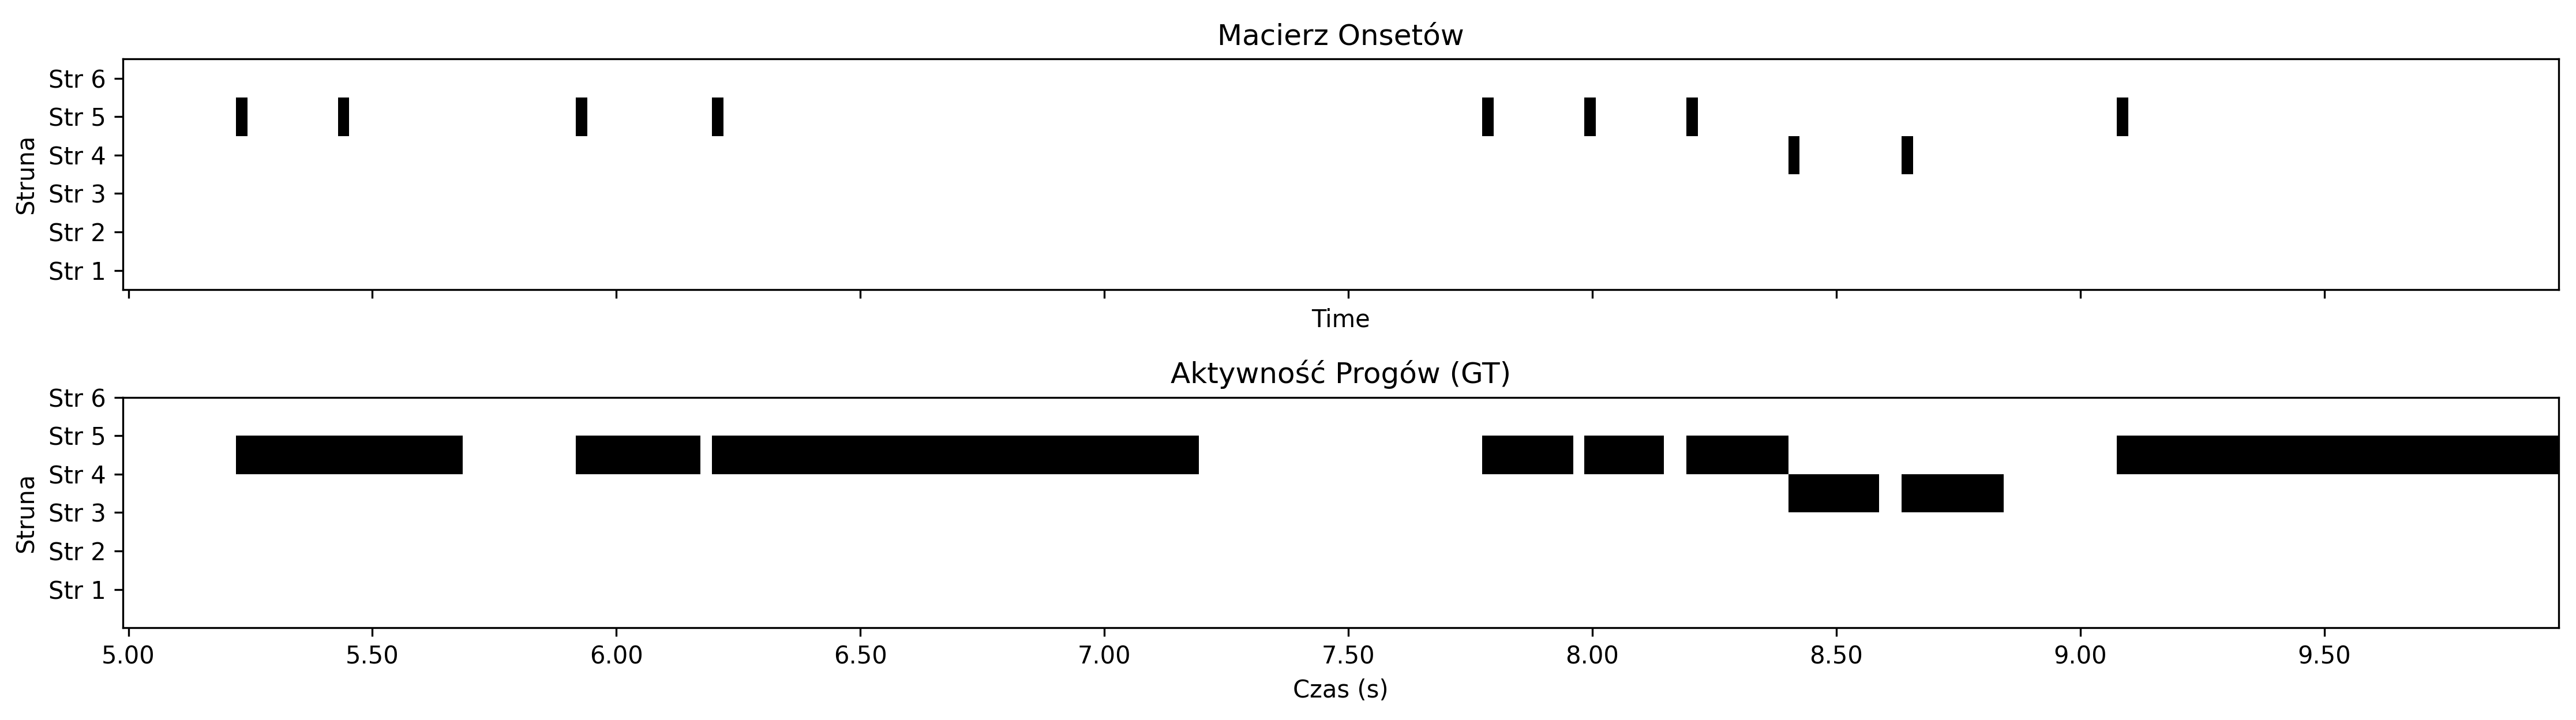
\includegraphics[width=\textwidth]{fig/fig_3_1.png}
    \caption{Wizualizacja etykiet ramkowych dla fragmentu utworu. Górny panel przedstawia macierz onsetów, gdzie pionowe linie oznaczają moment rozpoczęcia nuty na danej strunie. Dolny panel pokazuje macierz aktywności progów, gdzie czarne obszary reprezentują czas trwania dźwięku na danej strunie.}
    \label{fig:piano_roll_labels}
\end{figure}

\subsubsection{Komponent zbioru danych i augmentacja}
\label{sssec:komponent_zbioru_danych_augmentacja}

Dedykowany komponent zbioru danych, zgodny ze standardowym interfejsem frameworka PyTorch, odpowiada za ładowanie i~przygotowywanie danych dla modelu. Kluczową decyzją projektową jest rozróżnienie sposobu przygotowania danych dla poszczególnych podzbiorów. Dla zbiorów walidacyjnego i~testowego, cechy są obliczane jednorazowo i~zapisywane na dysku. Zapewnia to pełną powtarzalność i~spójność procesu ewaluacji~– model jest zawsze testowany na identycznych, niezmienionych danych. Natomiast dla zbioru treningowego, spektrogramy CQT są generowane ,,w locie'' z~surowych plików audio w~każdej epoce treningu. Takie podejście, choć wolniejsze, umożliwia stosowanie dynamicznej augmentacji na poziomie sygnału audio, co znacząco zwiększa różnorodność danych treningowych.

Wstępna walidacja jakościowa oraz analiza wyników z~początkowych eksperymentów wykazały, że model wytrenowany wyłącznie na czystych, studyjnych nagraniach z~GuitarSet wykazywał niską zdolność do generalizacji na sygnały audio, które zawierały typowe niedoskonałości nagrań amatorskich. W~odpowiedzi na to wyzwanie, przyjęto strategię, której celem jest poprawa odporności i~zdolności generalizacyjnych modelu poprzez uczenie go na danych symulujących realistyczne warunki. W~tym celu zaimplementowano rozbudowany potok augmentacji, wprowadzający do danych treningowych kontrolowane zakłócenia. Zastosowane techniki augmentacji obejmują:

\begin{itemize}
    \item \textbf{Augmentacje audio} (stosowane do surowego sygnału przed obliczeniem CQT)~\autocite{KlapuriDavy2006SignalProcessing, Benetos2019AutomaticMusicTranscription}:
    \begin{itemize}
        \item Rozciąganie w~czasie (ang. \textit{time stretching}): modyfikuje tempo nagrania w~zdefiniowanym zakresie, z~odpowiednią korektą czasów w~etykietach.
        \item Dodawanie szumu (ang. \textit{noise addition}): do sygnału dodawany jest szum o~losowo wybranej amplitudzie.
        \item Losowe wzmocnienie (ang. \textit{random gain}): amplituda sygnału jest mnożona przez losowy współczynnik, symulując zmiany dynamiki.
        \item Symulacja pogłosu pomieszczenia (ang. \textit{reverb}): W celu nauczenia modelu ignorowania akustyki pomieszczenia, do sygnału dodawany jest sztuczny pogłos. Jest on generowany poprzez operację splotu matematycznego z~syntetyczną odpowiedzią impulsową. Kluczowe parametry tego efektu, takie jak czas zanikania oraz natężenie, są losowane w~każdym kroku, co symuluje nagrania w~setkach różnych środowisk akustycznych – od małych, wytłumionych pokoi po większe przestrzenie z~wyraźnym echem.
        \item Symulacja charakterystyki mikrofonu (ang. \textit{EQ}): Aby naśladować działanie mikrofonów niższej jakości (np. w~laptopach), które słabo zbierają skrajne pasma częstotliwości, stosowany jest cyfrowy filtr pasmowo-przepustowy. Filtr ten ,,obcina'' najniższe (bas) i~najwyższe (sopran) częstotliwości, tworząc bardziej ,,pudełkowy'', skupiony w~środku dźwięk. Model uczy się w~ten sposób, że brak pełni brzmienia nie musi oznaczać braku nuty. Częstotliwości odcięcia filtru są losowane z~szerokiego zakresu, co symuluje całą gamę niedoskonałych urządzeń nagrywających.
        \item Symulacja przesterowania (ang. \textit{clipping}): W warunkach domowych łatwo jest ustawić zbyt wysoki poziom głośności nagrywania, co prowadzi do cyfrowego obcinania wierzchołków fali dźwiękowej. Aby przygotować model na takie sytuacje, wprowadzono augmentację, która celowo obcina amplitudę sygnału po przekroczeniu pewnego progu. Uczy to model rozpoznawania nut nawet wtedy, gdy ich sygnał jest zniekształcony w~ten sposób. Próg, przy którym następuje obcięcie, jest losowany, co naśladuje różne stopnie przesterowania sygnału.
    \end{itemize}
    \item \textbf{Augmentacja spektrogramu} (SpecAugment)~\autocite{Park2019SpecAugment}: stosowana do wygenerowanych spektrogramów (Mel lub CQT). Polega na losowym maskowaniu pewnych fragmentów spektrogramu:
    \begin{itemize}
        \item Maskowanie w~dziedzinie czasu (ang. \textit{Time Masking}): Losowe zakrywanie pewnej liczby kolejnych ramek czasowych.
        \item Maskowanie w~dziedzinie częstotliwości (ang. \textit{Frequency Masking}): Losowe zakrywanie pewnego zakresu pasm częstotliwości.
    \end{itemize}
\end{itemize}
Podczas każdej epoki treningu model otrzymuje próbki poddane unikalnej, losowej kombinacji powyższych transformacji. Takie podejście zmusza model do nauki bardziej niezmiennych cech sygnału, co przekłada się na lepszą generalizację.

\subsubsection{Przetwarzanie wsadowe i walidacja danych}
\label{sssec:przetwarzanie_wsadowe_walidacja}

W celu efektywnego treningu modelu, próbki danych są grupowane we wsady (ang. \textit{batches}). Ponieważ poszczególne nagrania w~zbiorze danych mają różną długość, zaimplementowano mechanizm dopełniania (ang. \textit{padding}). Dedykowana funkcja agregująca, używana przez mechanizm ładowania danych, uzupełnia tensory cech i~etykiet w~ramach danego wsadu do długości najdłuższej sekwencji w~tym wsadzie. Proces ten wykorzystuje standardowe narzędzia frameworka PyTorch.

System wyposażono również w~zestaw narzędzi diagnostycznych, służących do weryfikacji poprawności i~spójności przetworzonych danych. Funkcje te sprawdzają, czy kształty i~typy danych tensorów (np. CQT, Mel, etykiet onsetów i~progów) są zgodne z~oczekiwaniami zdefiniowanymi w~konfiguracji, oraz czy wartości w~tensorach mieszczą się w~oczekiwanych zakresach (np. czy są to wartości binarne, czy nie występują wartości nieokreślone). Umożliwia to przeprowadzenie pełnej walidacji na całym zbiorze danych, agregując statystyki i~generując podsumowanie.

%%
\subsection{Model Transkrypcji (CRNN)}
\label{ssec:model_transkrypcji_crnn}

Sercem systemu transkrypcji jest konwolucyjno-rekurencyjna sieć neuronowa (CRNN), zaimplementowana w~frameworku PyTorch. Architektura ta, przedstawiona na rysunku~\ref{fig:crnn_architecture}, została zaprojektowana z~myślą o~przetwarzaniu dwuwymiarowych reprezentacji czasowo-częstotliwościowych (głównie CQT) i~modelowaniu zależności czasowych. Model składa się z~trzech głównych bloków:
\begin{itemize}
    \item \textbf{Frontend konwolucyjny (CNN)}: Ta część jest odpowiedzialna za ekstrakcję hierarchicznych cech z~wejściowego spektrogramu. Składa się z~sekwencji pięciu warstw konwolucyjnych 2D (\texttt{Conv2d}) z~filtrami o~rozmiarze 3x3, po których następują warstwy normalizacji wsadowej, funkcje aktywacji ReLU oraz warstwy max-pooling redukujące wymiarowość map cech~\autocite{Wiggins2019TabCNN, BurletHindle2017IsolatedGuitarTranscription}. Liczba filtrów w~kolejnych warstwach jest konfigurowalna.
    \item \textbf{Backend rekurencyjny (RNN)}: Złożony z~dwukierunkowych warstw rekurencyjnych. Zadaniem tego bloku jest modelowanie zależności czasowych w~sekwencjach cech wyekstrahowanych przez CNN~\autocite{Benetos2019AutomaticMusicTranscription}. Dwukierunkowość pozwala na analizę każdej ramki w~kontekście zarówno przeszłych, jak i~przyszłych zdarzeń, co jest korzystne dla precyzji transkrypcji~\autocite{Hawthorne2018Onsets, KlapuriDavy2006SignalProcessing}. W~projekcie wykorzystano głównie bramkowane jednostki rekurencyjne (GRU, ang. \textit{Gated Recurrent Unit})~\autocite{Chung2014GRU}. Jednostki GRU, posiadając prostszą architekturę od tradycyjnych LSTM (ang. \textit{Long Short-Term Memory}), są często bardziej wydajne obliczeniowo, oferując przy tym porównywalną skuteczność w~modelowaniu sekwencji. Kluczowe parametry RNN, takie jak rozmiar stanu ukrytego, liczba warstw oraz współczynnik dropout dla regularyzacji, są konfigurowalnymi hiperparametrami.
    \item \textbf{Warstwy Wyjściowe}: Przetworzone przez RNN sekwencje cech są następnie podawane na dwie oddzielne, w~pełni połączone warstwy liniowe. Jedna warstwa (\texttt{onset\_fc}) generuje logity dla predykcji onsetów dla każdej z~sześciu strun. Druga warstwa (\texttt{fret\_fc}) generuje logity dla predykcji klas progów (włączając klasę ciszy) dla każdej struny. Takie podejście wielozadaniowe, gdzie model uczy się jednocześnie detekcji zdarzeń i~klasyfikacji stanów, jest inspirowane pracą "Onsets and Frames"~\autocite{Hawthorne2018Onsets}.
\end{itemize}
System zawiera również funkcję pomocniczą do ładowania zapisanego stanu modelu z~pliku, tworząc nową instancję modelu z~odpowiednimi parametrami i~wczytując do niej zapisane wagi.

\begin{figure}[H]
    \centering
    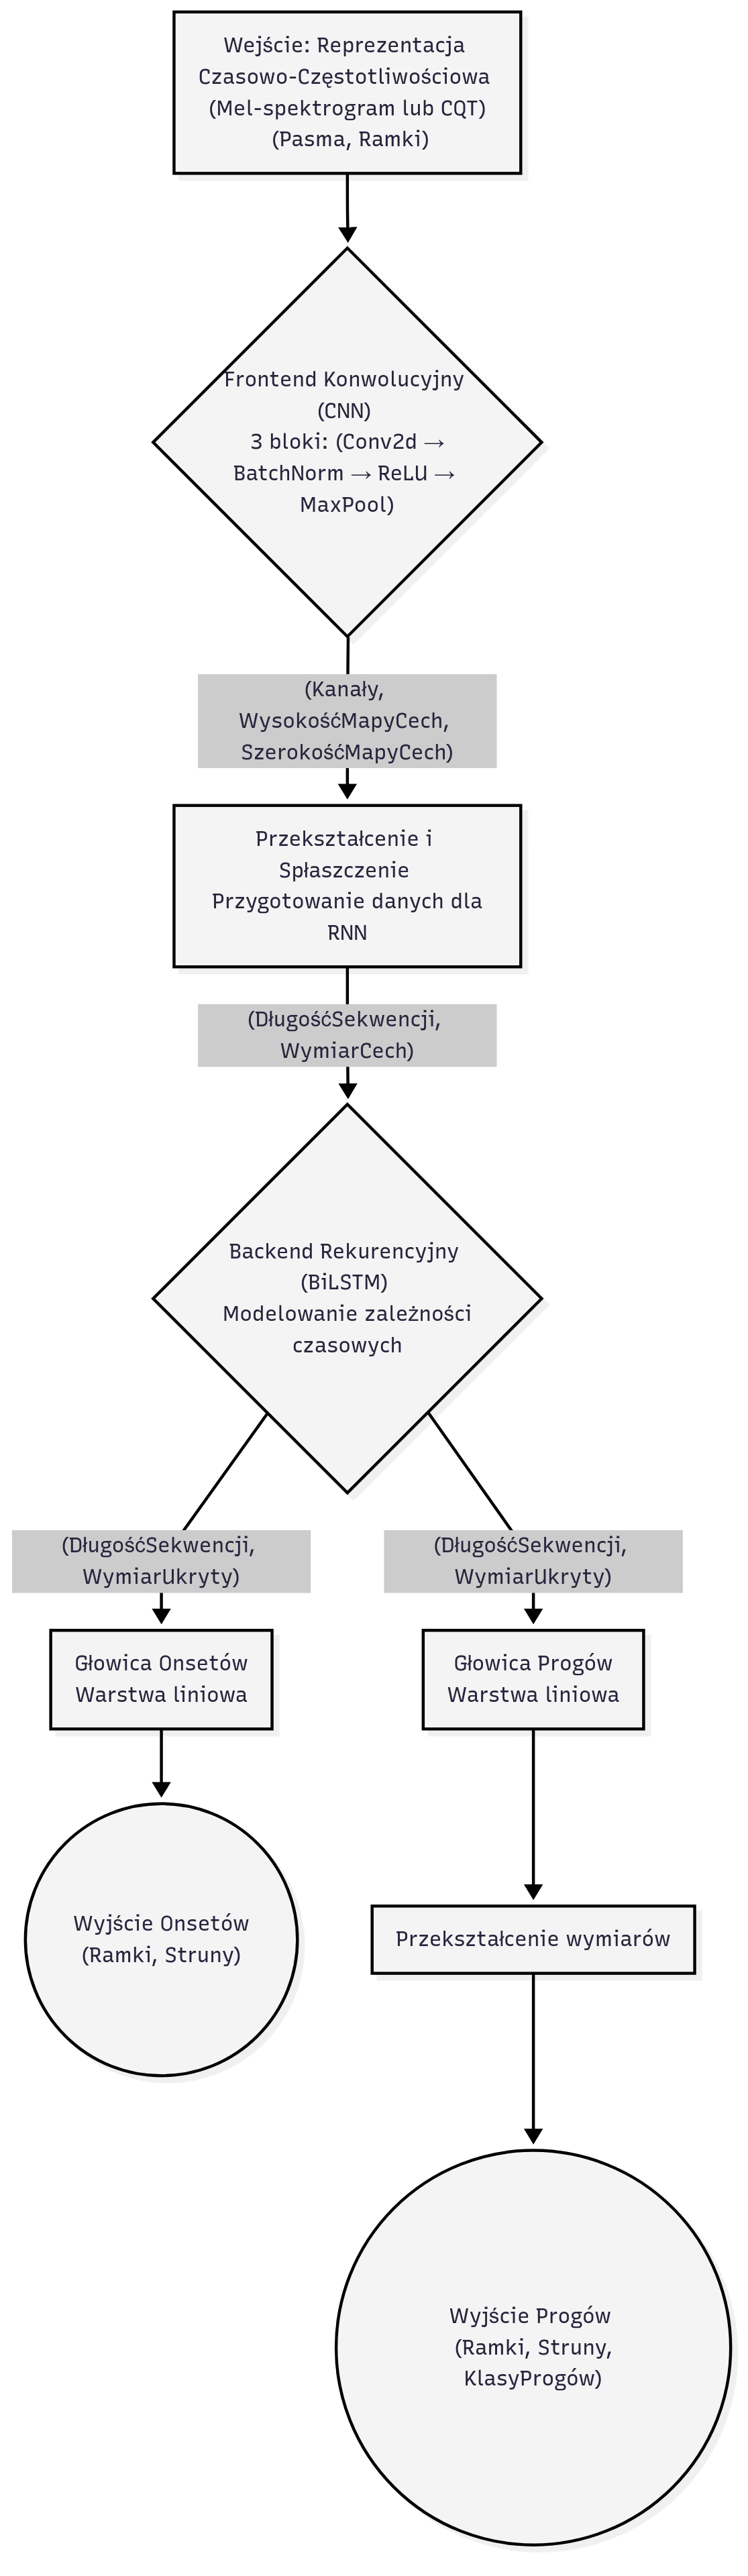
\includegraphics[width=0.4\textwidth]{fig/fig_3_2.png}
    \caption{Schemat architektury zaimplementowanego modelu CRNN. Przedstawia przepływ danych od wejściowego tensora spektrogramu, przez frontend konwolucyjny, backend rekurencyjny, aż po rozdzielenie na dwie głowice wyjściowe dla predykcji onsetów i~progów.}
    \label{fig:crnn_architecture}
\end{figure}

\subsection{Proces Treningu Modelu}
\label{ssec:proces_treningu_modelu}

Proces treningu modelu jest zarządzany przez dedykowany moduł, który orkiestruje cały cykl dla pojedynczego zestawu hiperparametrów.

\subsubsection{Inicjalizacja i Pętla Treningowa}
\label{sssec:inicjalizacja_petla_treningowa}

Dla każdego przebiegu w~ramach przeszukiwania hiperparametrów tworzony jest unikalny katalog na artefakty. Następnie inicjalizowany jest model CRNN, funkcja straty oraz optymalizator. Zdecydowano się na użycie optymalizatora AdamW~\autocite{Loshchilov2019AdamW}. Jest to udoskonalona wersja popularnego optymalizatora Adam, która inaczej implementuje mechanizm regularyzacji (zaniku wag, ang. \textit{weight decay}). W~AdamW zanik wag jest oddzielony od kroku aktualizacji gradientu, co prowadzi do bardziej stabilnego treningu i~lepszej generalizacji modelu w~porównaniu do standardowej implementacji L2 w~Adam. Początkowy współczynnik uczenia jest kluczowym hiperparametrem. Na podstawie tych parametrów inicjowany jest również, opcjonalnie, mechanizm harmonogramowania współczynnika uczenia (np. ReduceLROnPlateau), który redukuje współczynnik uczenia o~konfigurowalny czynnik, gdy metryka walidacyjna przestaje się poprawiać przez określoną liczbę epok.

Główna pętla treningowa iteruje przez zdefiniowaną liczbę epok. W~każdej epoce wykonywane są dwie fazy:
\begin{itemize}
    \item \textbf{Faza treningowa}: Model jest ustawiany w~tryb treningowy. Dla każdego wsadu danych ze zbioru treningowego zerowane są gradienty, wykonywane jest przejście w~przód przez model, obliczana jest złożona funkcja straty, a~następnie wykonywana jest propagacja wsteczna i~aktualizacja wag modelu przez optymalizator.
    \item \textbf{Faza walidacyjna}: Model jest ustawiany w~tryb ewaluacyjny, a~obliczanie gradientów jest wyłączane. Dla każdego wsadu danych ze zbioru walidacyjnego wykonywane jest przejście w~przód, obliczana jest funkcja straty oraz szeroki zestaw metryk wydajności.
\end{itemize}
Wszystkie straty i~metryki są zapisywane w~historii treningu. Postępy są logowane do pliku tekstowego oraz wyświetlane na konsoli. Stosowany jest mechanizm wczesnego zatrzymywania (ang. \textit{early stopping}), który przerywa trening, jeśli śledzona metryka walidacyjna nie poprawia się przez zadaną, większą liczbę epok, aby zapobiec przeuczeniu i~zaoszczędzić zasoby obliczeniowe~\autocite{Benetos2019AutomaticMusicTranscription}. Najlepszy model (na podstawie metryki walidacyjnej) jest zapisywany. Na koniec generowany jest wykres historii treningu. Zastosowano również techniki regularyzacji w~celu zapobiegania przeuczeniu: dropout w~warstwach LSTM~\autocite{Chung2014GRU, KlapuriDavy2006SignalProcessing} oraz regularyzację L2 (weight decay)~\autocite{Loshchilov2019AdamW, KlapuriDavy2006SignalProcessing}. Wartość współczynnika zaniku wag jest kolejnym istotnym hiperparametrem.

\subsubsection{Funkcja Straty i Próg Decyzyjny}
\label{sssec:funkcja_straty_prog}

Zastosowano złożoną funkcję straty ($\mathcal{L}_{\text{total}}$), która jest ważoną sumą dwóch komponentów: straty dla predykcji onsetów ($\mathcal{L}_{\text{onset}}$) oraz straty dla predykcji progów ($\mathcal{L}_{\text{fret}}$), co przedstawia wzór~\ref{eq:combined_loss}:
\begin{equation}
    \mathcal{L}_{\text{total}} = w_{\text{onset}} \cdot \mathcal{L}_{\text{onset}} + w_{\text{fret}} \cdot \mathcal{L}_{\text{fret}}
    \label{eq:combined_loss}
\end{equation}
gdzie $w_{\text{onset}}$ i~$w_{\text{fret}}$ to wagi poszczególnych komponentów straty. Wartość $w_{\text{onset}}$ jest konfigurowalnym hiperparametrem, natomiast $w_{\text{fret}}$ przyjęto jako 1.0.

Stratę $\mathcal{L}_{\text{onset}}$ oblicza się przy użyciu ważonej binarnej entropii krzyżowej z~logitami (\texttt{BCEWithLogitsLoss}), aby przeciwdziałać niezbalansowaniu klas (onety są zdarzeniami rzadkimi w~porównaniu do braku onsetu). Waga dla pozytywnych przykładów (onety) jest określana przez konfigurowalny hiperparametr. Dla pojedynczej struny $s$ i~ramki $t$, strata onsetu jest dana wzorem:
\begin{equation}
    \mathcal{L}_{\text{onset}_{s,t}} = - [w_{\text{pos}} \cdot y_{s,t}^{\text{onset}} \log(\sigma(\hat{z}_{s,t}^{\text{onset}})) + (1-y_{s,t}^{\text{onset}})\log(1-\sigma(\hat{z}_{s,t}^{\text{onset}}))]
    \label{eq:onset_loss_formula}
\end{equation}
gdzie $y_{s,t}^{\text{onset}} \in \{0,1\}$ to etykieta referencyjna, $\hat{z}_{s,t}^{\text{onset}}$ to logit wyjściowy modelu dla onsetu, $\sigma(\cdot)$ to funkcja sigmoid, a~$w_{\text{pos}}$ to waga dla pozytywnych przykładów. Całkowita $\mathcal{L}_{\text{onset}}$ jest średnią $\mathcal{L}_{\text{onset}_{s,t}}$ po wszystkich strunach i~ramkach wsadu, z~uwzględnieniem maskowania dla ramek dopełniających.

Stratę $\mathcal{L}_{\text{fret}}$ oblicza się przy użyciu standardowej entropii krzyżowej (\texttt{CrossEntropyLoss}) dla klasyfikacji progów na każdej strunie. Wykorzystuje się ignorowanie określonego indeksu (\texttt{ignore\_index}) do pomijania wartości dopełniających. Dla pojedynczej struny $s$ i~ramki $t$:
\begin{equation}
    \mathcal{L}_{\text{fret}_{s,t}} = - \sum_{c=0}^{N_{\text{klas progu}}-1} y_{s,t,c}^{\text{fret}} \log(p_{s,t,c}^{\text{fret}})
    \label{eq:fret_loss_formula}
\end{equation}
gdzie $y_{s,t,c}^{\text{fret}}$ jest wskaźnikiem (0 lub 1), czy klasa progu $c$ jest poprawna, a~$p_{s,t,c}^{\text{fret}}$ jest prawdopodobieństwem predykcji klasy $c$ (wyjście funkcji softmax). Całkowita $\mathcal{L}_{\text{fret}}$ jest średnią $\mathcal{L}_{\text{fret}_{s,t}}$ po wszystkich strunach i~ramkach.

W celu zapewnienia szybkości i~spójności procesu treningu, podczas fazy walidacyjnej w~każdej epoce stosowany jest stały próg decyzyjny dla predykcji onsetów. Predykcja jest uznawana za pozytywną (wystąpienie onsetu), jeśli zwrócone przez model prawdopodobieństwo przekracza wartość 0.5. Bardziej zaawansowany proces wyszukiwania optymalnego progu, który maksymalizuje docelową metrykę (np. TDR F1-score), jest celowo odroczony i~wykonywany jest tylko jednokrotnie, w~ramach finalnej analizy na zbiorze testowym, co zostało szczegółowo opisane w~sekcji~\ref{ssec:ewaluacja_generowanie_wynikow_rozdzial}.

\subsection{Ewaluacja i Generowanie Wyników}
\label{ssec:ewaluacja_generowanie_wynikow_rozdzial}

Po zakończeniu treningu, najlepszy model jest poddawany finalnej ewaluacji na zbiorze testowym. System umożliwia również generowanie wyników w~formatach ułatwiających analizę jakościową.

\subsubsection{Konwersja Predykcji na Nuty i Metryki Ewaluacyjne}
\label{sssec:konwersja_metryki_ewaluacyjne}

Ramkowe predykcje modelu, składające się z~prawdopodobieństw onsetów i~rozkładów prawdopodobieństwa dla klas progów, są w~pierwszym kroku przekształcane w~listę dyskretnych zdarzeń nutowych. Proces ten, zrealizowany w~module \texttt{note\_conversion\_utils.py}, iteruje po każdej z~sześciu strun, wykorzystując logikę maszyny stanów do identyfikacji początków i~końców nut. Wykrycie onsetu (prawdopodobieństwo powyżej progu) dla aktywnego progu inicjuje nową nutę, która jest kontynuowana do momentu spełnienia warunku terminacji (np. kolejny onset na tej samej strunie). Wynikiem jest symboliczna reprezentacja transkrypcji, gotowa do oceny ilościowej.

Podejście do ewaluacji opiera się na zestawie trzech komplementarnych metryk, które oceniają różne aspekty jakości transkrypcji, od precyzji czasowej po poprawność tonalną. Wszystkie metryki bazują na fundamentalnych pojęciach:
\begin{itemize}
    \item \textbf{True Positives (TP):} Poprawnie zidentyfikowane zdarzenia (nuty, onety, aktywne ramki).
    \item \textbf{False Positives (FP):} Zdarzenia przewidziane przez model, które nie mają odpowiednika w~danych referencyjnych (,,fałszywe alarmy'').
    \item \textbf{False Negatives (FN):} Zdarzenia obecne w~danych referencyjnych, które zostały pominięte przez model.
\end{itemize}
Na ich podstawie obliczane są standardowe wskaźniki: Precyzja, Czułość oraz miara F1-Score, zdefiniowane następującymi wzorami:
\begin{equation}
    \text{Precyzja} = \frac{TP}{TP + FP}
    \label{eq:precision}
\end{equation}
\begin{equation}
    \text{Czułość (Recall)} = \frac{TP}{TP + FN}
    \label{eq:recall}
\end{equation}
\begin{equation}
    \text{F1-Score} = 2 \cdot \frac{\text{Precyzja} \cdot \text{Czułość}}{\text{Precyzja} + \text{Czułość}}
    \label{eq:f1_score}
\end{equation}

Kluczowe jest jednak to, jak TP, FP i~FN są definiowane dla każdej z~poszczególnych metryk.

\paragraph{Metryka Główna: Tablature Detection Rate (TDR)}
TDR jest najważniejszą metryką, oceniającą finalną jakość wygenerowanej tabulatury. Nuta jest uznawana za poprawną (TP) tylko wtedy, gdy predykcja jest zgodna z~adnotacją referencyjną we wszystkich trzech wymiarach:
\begin{itemize}
    \item \textbf{Zgodność Czasu Rozpoczęcia:} Czas onsetu predykcji mieści się w~oknie tolerancji $\pm$50 ms wokół onsetu referencyjnego.
    \item \textbf{Zgodność Struny:} Predykcja i~adnotacja wskazują na ten sam numer struny.
    \item \textbf{Zgodność Progu:} Predykcja i~adnotacja wskazują na ten sam numer progu.
\end{itemize}
Każda przewidziana nuta, która nie spełnia tych kryteriów, jest liczona jako FP, a~każda nuta referencyjna, dla której nie znaleziono dopasowania, jako FN~\autocite{Wiggins2019TabCNN}.

\paragraph{Metryka Diagnostyczna Timingu: Onset F1-Score}
Ta metryka w~izolacji ocenia zdolność modelu do precyzyjnego lokalizowania w~czasie momentów rozpoczęcia dźwięków. Do jej obliczenia wykorzystano standardową w~badaniach MIR bibliotekę \texttt{mir\_eval}. Zdarzenie jest tu uznawane za poprawne (TP), jeśli spełniony jest tylko jeden warunek:
\begin{itemize}
    \item \textbf{Zgodność Czasu Rozpoczęcia:} Czas onsetu predykcji mieści się w~oknie tolerancji $\pm$50 ms wokół onsetu referencyjnego.
\end{itemize}
Poprawność progu i~struny jest na tym etapie ignorowana. Implementacja w~\texttt{mir\_eval} zapewnia poprawne, jedno-do-jednego dopasowanie zdarzeń, co jest kluczowe dla wiarygodności tej metryki~\autocite{Benetos2019AutomaticMusicTranscription}.

\paragraph{Metryka Diagnostyczna Wysokości Dźwięku: MPE F1-Score}
Metryka Multi-Pitch Estimation (MPE) na poziomie ramek ocenia, czy model poprawnie rozpoznaje, jaki dźwięk (próg) jest aktywny w~danym, krótkim momencie. W~przeciwieństwie do TDR, nie analizuje ona nut jako zdarzeń, lecz ciągłą aktywność dźwięków. Dla każdej ramki czasowej i~każdej struny:
\begin{itemize}
    \item \textbf{TP:} Ramka, w~której zarówno etykieta referencyjna, jak i~predykcja wskazują na aktywny dźwięk (nie ciszę) ORAZ numer progu jest w~nich identyczny.
    \item \textbf{FP:} Ramka, w~której model przewidział aktywny dźwięk, podczas gdy w~etykiecie była cisza, LUB model przewidział zły numer progu dla aktywnej nuty.
    \item \textbf{FN:} Ramka, w~której etykieta wskazywała na aktywny dźwięk, podczas gdy model przewidział ciszę, LUB model przewidział zły numer progu dla aktywnej nuty.
\end{itemize}
Ta metryka pozwala precyzyjnie zdiagnozować problemy z~rozpoznawaniem wysokości dźwięków, niezależnie od dokładności detekcji onsetów~\autocite{Bittner2022BasicPitch}.

\subsubsection{Generowanie Wyników i Analiza Końcowa}
\label{sssec:generowanie_wynikow_analiza_koncowa}

Finalny etap pracy z~modelem obejmuje szczegółową analizę jego działania na niewidzianych wcześniej danych testowych oraz generowanie czytelnych dla człowieka wyników. W~tym celu, po zakończeniu całego procesu przeszukiwania hiperparametrów i~wyborze najlepszego modelu (na podstawie metryki walidacyjnej), uruchamiany jest dedykowany skrypt analityczny.

Proces ten przebiega w~kilku krokach. Najpierw, najlepszy model jest uruchamiany na całym zbiorze testowym w~celu zebrania kompletnych predykcji (prawdopodobieństw onsetów i~macierzy progów) dla każdego utworu. Następnie, system przeprowadza procedurę optymalizacyjną, aby znaleźć optymalny próg decyzyjny dla onsetów, który maksymalizuje uśrednioną metrykę TDR F1-score na zbiorze testowym.

Kluczowym elementem analizy jest ocena jakości transkrypcji dla każdego pliku z~osobna. Używając znalezionego optymalnego progu, system oblicza TDR F1-score dla każdego utworu testowego, a~następnie tworzy ranking plików od tych z~najlepszym wynikiem (najwyższy F1-score) do tych z~najgorszym. Na podstawie tego rankingu, generowane są pliki tabulatur w~formacie tekstowym (ASCII) dla kilku najlepszych i~kilku najgorszych przypadków. Takie podejście pozwala na dogłębną, jakościową analizę błędów modelu, ułatwiając zrozumienie, w~jakich warunkach radzi on sobie najlepiej, a~gdzie popełnia najwięcej błędów.

\subsection{Wizualizacja}
\label{ssec:wizualizacja}

System zawiera zestaw funkcji do tworzenia różnego rodzaju wykresów przy użyciu biblioteki Matplotlib. Umożliwiają one wizualizację:
\begin{itemize}
    \item Spektrogramów wejściowych (Mel lub CQT).
    \item Etykiet i~predykcji onsetów w~formie grafu typu "piano roll".
    \item Etykiet i~predykcji progów w~formie kolorowej mapy.
    \item Zbiorczych wykresów dla pojedynczych próbek, pokazujących spektrogram oraz odpowiadające mu etykiety i~predykcje.
    \item Ewolucji strat i~metryk wydajności w~kolejnych epokach treningu.
\end{itemize}
Te narzędzia wizualizacyjne są wykorzystywane zarówno do weryfikacji poprawności danych, jak i~do analizy wyników działania modelu i~procesu treningu.

\section{Uzasadnienie Wyboru Zastosowanych Metod, Algorytmów i Narzędzi}
\label{sec:uzasadnienie_wyboru_metod_fakt}

W tej sekcji przedstawiono uzasadnienie decyzji dotyczących wyboru konkretnych metod, algorytmów i~narzędzi programistycznych, opierając się na przedstawionych faktach implementacyjnych.

\subsection{Wybór Reprezentacji Czasowo-Częstotliwościowych}
\label{ssec:uzasadnienie_reprezentacji_wybor_fakt}

Decyzja o~zaimplementowaniu i~umożliwieniu porównania mel-spektrogramów oraz spektrogramów CQT jest motywowana chęcią empirycznej weryfikacji skuteczności tych dwóch popularnych reprezentacji w~kontekście GTT. Mel-spektrogramy są standardem w~wielu zadaniach MIR ze względu na ich psychoakustyczną motywację~\autocite{Benetos2019AutomaticMusicTranscription, KlapuriDavy2006SignalProcessing}. Z~kolei CQT, z~logarytmiczną skalą częstotliwości, jest teoretycznie lepiej dopasowana do natury muzyki i~może ułatwiać modelom CNN naukę cech istotnych dla transkrypcji gitarowej~\autocite{Wiggins2019TabCNN, Zang2023SynthTab, KlapuriDavy2006SignalProcessing}. Możliwość eksperymentowania z~obiema reprezentacjami w~ramach jednego systemu jest jego istotną zaletą badawczą.

\subsection{Architektura CRNN jako Model Transkrypcji}
\label{ssec:uzasadnienie_crnn_wybor_fakt}

Wybór architektury CRNN, łączącej konwolucyjny front-end (TabCNN) z~rekurencyjnym back-endem (LSTM), jest uzasadniony jej udokumentowaną skutecznością w~zadaniach transkrypcji muzycznej~\autocite{Hawthorne2018Onsets, Wiggins2019TabCNN}. CNN efektywnie ekstrahują cechy z~dwuwymiarowych spektrogramów, podczas gdy dwukierunkowe LSTM modelują zależności czasowe w~tych cechach. Takie połączenie pozwala na kompleksową analizę sygnału audio. Architektura ta oferuje dobry kompromis między zdolnościami modelowania a~złożonością obliczeniową, co jest istotne przy ograniczonych zasobach i~rozmiarze zbioru danych, w~porównaniu do bardziej zasobożernych modeli, np. opartych w~całości na Transformerach~\autocite{Hawthorne2021Seq2SeqTranscription}. Zastosowanie optymalizatora AdamW zamiast Adam jest motywowane jego lepszą obsługą zaniku wag, co często przekłada się na lepszą generalizację modelu~\autocite{Loshchilov2019AdamW}.

\subsection{Wykorzystane Biblioteki Programistyczne}
\label{ssec:uzasadnienie_bibliotek_wybor_fakt}

Dobór narzędzi programistycznych odzwierciedla aktualne standardy w~badaniach z~zakresu MIR i~uczenia maszynowego.
\begin{itemize}
    \item \textbf{PyTorch} został wybrany jako główny framework do głębokiego uczenia ze względu na jego elastyczność, dynamiczne grafy obliczeniowe oraz bogaty ekosystem narzędzi wspierających rozwój modeli uczenia maszynowego~\autocite{Paszke2019PyTorch}.
    \item \textbf{Librosa} jest standardową biblioteką do analizy sygnałów audio i~muzyki w~Pythonie, dostarczającą implementacje funkcji do wczytywania audio, ekstrakcji cech (STFT, mel-spektrogramy, CQT) oraz augmentacji~\autocite{McFee2022Librosa}.
    \item \textbf{Mirdata} ułatwia standaryzowaną pracę ze zbiorami danych MIR, takimi jak GuitarSet, promując powtarzalność badań~\autocite{Bittner2022BasicPitch}.
    \item Inne biblioteki, takie jak NumPy, Scikit-learn, Matplotlib, JAMS i~PrettyMIDI, dostarczają niezbędnych narzędzi na różnych etapach projektu, od operacji numerycznych, przez podział danych i~wizualizację, po pracę z~adnotacjami i~generowanie plików MIDI. Do implementacji zaawansowanych augmentacji audio wykorzystano również bibliotekę \textbf{SciPy} ze względu na jej wydajne i~stabilne funkcje przetwarzania sygnałów, w~tym filtry cyfrowe i~operację splotu.
\end{itemize}
Korzystanie z~tych sprawdzonych narzędzi pozwoliło na skupienie się na aspektach badawczych projektu.

\section{Podsumowanie Rozdziału}
\label{sec:podsumowanie_rozdzialu_3_fakt}

W niniejszym rozdziale szczegółowo przedstawiono projekt i~implementację autorskiego systemu do transkrypcji gitarowej. Omówiono jego architekturę, której trzon stanowi konwolucyjno-rekurencyjna sieć neuronowa (CRNN), uzasadniając jej wybór zdolnością do jednoczesnego przetwarzania cech czasowo-częstotliwościowych i~modelowania sekwencji. Kluczowym elementem przedstawionego rozwiązania, stanowiącym odpowiedź na wyzwania związane z~przetwarzaniem nagrań amatorskich, jest zaawansowana strategia augmentacji danych. W rozdziale opisano, jak odejście od standardowych technik na rzecz celowego symulowania niedoskonałości sygnału – takich jak pogłos, zniekształcenia charakterystyki mikrofonu czy przesterowanie – pozwoliło na zbudowanie modelu o~większej odporności i~zdolności do generalizacji. Zaprezentowano również kompletny potok przetwarzania, od przygotowania danych ze zbioru GuitarSet, poprzez wielozadaniowy proces treningu, aż po kompleksowy system ewaluacji oparty na metrykach branżowych. Zaimplementowany system, ze szczególnym uwzględnieniem jego innowacyjnego podejścia do augmentacji, stanowi w~pełni przygotowaną i~uzasadnioną teoretycznie platformę, gotową do przeprowadzenia finalnych badań eksperymentalnych opisanych w~kolejnym rozdziale.
